% !TEX program = xelatex
% A题：自来水厂水质预测与评估 - 数学建模竞赛论文
\documentclass[12pt,a4paper]{ctexart}

% ===== Packages =====
\usepackage[top=2.5cm,bottom=2.5cm,left=2.5cm,right=2.5cm]{geometry}
\usepackage{amsmath,amssymb,amsfonts}
\usepackage{graphicx,subfig}
\usepackage{booktabs,tabularx,array}
\usepackage{hyperref,xcolor}
\usepackage{caption,float}
\usepackage{fancyhdr}

% ===== Settings =====
\hypersetup{colorlinks=true,linkcolor=blue,citecolor=blue,urlcolor=blue}
\renewcommand{\figurename}{\textbf{图}}
\renewcommand{\tablename}{\textbf{表}}
\captionsetup{font=small,labelfont=bf}
\renewcommand{\thesubfigure}{(\alph{subfigure})}
\setlength{\parindent}{2em}
\setlength{\parskip}{3pt}
\fancypagestyle{plain}{\fancyhf{}\fancyfoot[C]{\thepage}}
\pagestyle{plain}

% ===== Title =====
\title{\textbf{\heiti\zihao{2} 自来水厂水质预测与评估}}
\author{\zihao{4} 参赛队号: XXXXXX}
\date{}

\begin{document}
\maketitle
\thispagestyle{empty}

% ============================================================
% ABSTRACT
% ============================================================
\begin{center}
\zihao{4}\heiti\textbf{摘\quad 要}
\end{center}

\noindent 优质自来水供应是城市发展和公共健康的核心保障，自来水厂面临原水水质波动和工艺控制滞后两大挑战，精准的水质预测与风险评估对保障供水安全具有重要意义。本文基于某自来水厂连续15个月的高频监测数据（每2小时一次，共5460条记录，涵盖21个水质和工艺参数），围绕出水浊度(NTU)预测与水质风险评估，构建了从特征筛选、动态建模到风险评价的完整分析框架。

针对问题1，提出\textbf{MIFS-XGBoost-Stacking三层递进特征筛选与多模型融合预测框架}。第一层采用互信息(MI)过滤式方法初步筛选35个候选特征；第二层通过XGBoost嵌入式特征重要性排序，保留累积重要性超过92\%的特征子集；第三层利用排列重要性(Permutation Importance)验证特征贡献。在此基础上，构建以随机森林、GBDT、XGBoost、SVR为基学习器、Ridge回归为元学习器的Stacking集成模型。揭示了FILT.NTU(滤后水浊度)、时间周期特征(HOUR/MONTH)、原水浊度(RW\_NTU)及矾投加量(ALUM)等变量的核心作用。模型对2026年2月1日、10日、20日的出水NTU进行了预测，所有预测值均满足国标限值($\leq 1$ NTU)。

针对问题2，建立\textbf{TD-NARX(时滞非线性自回归外生模型)}。首先通过交叉相关函数(CCF)粗估各输入变量的时滞范围，随后采用遗传算法(GA)精搜异质时滞参数。模型识别出各输入变量的差异时滞：原水浊度(RW\_NTU)约2小时、原水pH(RW\_PH)约14小时、矾投加量(ALUM)约22小时、原水流量(RW\_FLOW)约24小时。NARX神经网络模型的测试集R$^2$=0.3415，RMSE=0.0523 NTU，验证了异质时滞假设的合理性。

针对问题3，构建\textbf{RTD-GBDT混合动态预测模型}。创新性地将化学反应工程中的停留时间分布(RTD)理论迁移至清水池水质建模，通过CSTR串联模型(串联级数$N=3$，平均停留时间$\tau=4$h)对滤后水浊度进行卷积平滑，得到物理约束特征；进而结合梯度提升决策树(GBDT)进行非线性预测。模型在测试集上R$^2$=0.7422，RMSE=0.0944 NTU。敏感性分析表明，矾投加量RTD卷积特征和原水浊度是影响预测精度的关键输入。对2026年2月1日、10日、20日7:00-19:00的逐小时预测结果均满足国标要求。

针对问题4，构建\textbf{FCE-SA(模糊综合评价-生存分析)双维度风险评价模型}。综合考虑NTU超标幅度($A$)与异常持续时长($D$)两个核心维度，建立加权综合评分($S=0.5A+0.3D+0.2F$)，采用模糊隶属度函数将2026年1-3月(共90天)划分为四个风险等级。评价结果显示：安全61天(67.8\%)、低风险25天(27.8\%)、中风险3天(3.3\%)、高风险1天(1.1\%)。3月12日出现最大超标事件(NTU达1.360，连续4小时超标)，为高风险日。风险日历和逐日评分曲线为水厂运维提供了直观的决策参考。

\vspace{1em}
\noindent\textbf{关键词：}自来水水质预测；NTU浊度建模；Stacking集成学习；TD-NARX时滞模型；RTD停留时间分布；模糊综合评价；数学建模

\newpage

% ============================================================
% TABLE OF CONTENTS
% ============================================================
\tableofcontents
\newpage

% ============================================================
% 1. INTRODUCTION
% ============================================================
\section{引言}

\subsection{研究背景与意义}

近年来，随着城市化进程加速和工业高质量发展，稳定优质的供水保障已成为城市吸引高端制造业、研发中心和国际企业落户的关键基础设施指标之一。国家"十五五"规划明确提出，确保城乡每个人都能获得基础、可靠的安全水源。自来水厂作为城市供水系统的核心节点，其生产过程涵盖取水、混凝、沉淀、过滤、消毒等多个环节，任一环节的波动都可能导致出厂水质不达标。

当前，自来水厂生产运营面临\textbf{两大核心挑战}：其一，原水水质波动（如雨季浊度剧增、pH值剧烈变化）导致后续工艺处理效果显著下降，甚至威胁出厂水质安全；其二，工艺控制存在明显滞后效应（如矾投加量调整后，滤后水浊度需数小时才能趋于稳定），传统经验式调控缺乏精准的预测与评估决策支持。在此背景下，构建数据驱动的水质预测与风险评估模型，实现从"被动响应"向"主动预警"的转变，具有重要的理论价值和工程实践意义。

从学术研究角度，水质预测方法经历了从经验统计模型到机理动力学模型，再到机器学习与混合建模的演进过程。传统方法如多元线性回归和ARIMA时间序列分析难以有效捕捉水处理过程中的非线性、多变量耦合和时滞特性。近年来，集成学习、深度学习和物理信息增强的混合建模方法逐渐成为主流研究方向。

\subsection{问题重述}

本文基于某自来水厂2025年1月至2026年3月连续15个月的运行监测数据（每2小时记录一次，涵盖原水水质、工艺过程参数、出厂水质及设备运行状态共21个指标），通过建立数学模型解决以下四个核心问题：

\begin{enumerate}
    \item 采用定量分析方法筛选影响自来水浊度(NTU)的主要因素，解释各因素的影响程度与作用方向，建立主要因素间的函数关系，并预测2026年2月1日、10日、20日的水浊度NTU，进行模型验证。
    \item 建立动态数学模型描述原水指标(R/W NTU、R/W pH)和操作变量(ALUM、R/W FLOW)如何影响滤后水浊度(FILT.NTU)，给出各输入变量的时滞参数，并对模型进行参数估计与验证。
    \item 结合质量守恒原理与数据驱动方法，建立混合动态模型预测未来1-12小时的出厂水浊度NTU，对2026年2月1日、10日、20日7:00-19:00进行预测，并进行敏感性分析。
    \item 以水浊度NTU为核心指标，结合超标幅度与异常持续时长，建立四级水质风险评价体系，对2026年1-3月进行分类评估，其中国标硬性约束为生活饮用水浊度限值$\leq 1$ NTU。
\end{enumerate}

\subsection{文献综述}

水质预测是环境工程和数学建模交叉领域的重要研究方向。国内外学者围绕水质参数预测、工艺过程建模和风险评估开展了大量研究。

在\textbf{水质预测方法}方面，研究经历了三个发展阶段。早期以统计方法为主，如Box-Jenkins时间序列分析、多元线性回归等。第二阶段以机理模型为核心，基于混凝动力学、沉淀理论和过滤方程建立确定性模型。近年来，机器学习方法成为主流，包括支持向量回归(SVR)、随机森林(RF)、梯度提升(GBDT/XGBoost)和深度学习(LSTM/GRU)等。

在\textbf{时滞建模}方面，传统方法多假设所有输入变量具有统一时滞，采用交叉相关分析(CCF)估计。近年来的研究开始关注异质时滞(heterogeneous time delay)建模，允许不同输入变量具有独立时滞参数，更符合实际物理过程。

在\textbf{混合建模}方面，物理信息增强的数据驱动方法(Physics-Informed Machine Learning)逐渐成为趋势，通过将物理约束（如质量守恒、停留时间分布）嵌入数据驱动模型，提升外推能力和物理一致性。

在\textbf{水质风险评价}方面，传统方法多基于单一阈值判别，近年来的研究开始引入模糊综合评价、灰色关联分析和贝叶斯网络等方法，实现更精细化的风险分级管理。

本文在前人研究基础上，提出了一套完整的"特征筛选—动态建模—混合预测—风险评价"分析框架，创新点包括：(1)三层递进特征筛选与多模型Stacking融合；(2)异质时滞NARX动态建模；(3)RTD理论向水质预测的跨领域迁移；(4)双维度模糊评价与生存分析的耦合应用。

\subsection{全文结构}

本文结构安排如下：第2节阐述模型假设与符号说明；第3-6节分别针对四个问题进行建模求解；第7节进行模型综合评价与讨论；第8节总结全文并提出展望。

\newpage

% ============================================================
% 2. MODEL ASSUMPTIONS AND NOTATIONS
% ============================================================
\section{模型假设与符号说明}

\subsection{模型假设}

\begin{enumerate}
    \item \textbf{数据代表性假设}：15个月的监测数据（含完整干湿季周期）能够充分反映水厂在不同原水水质、气候条件和运行策略下的动态响应特征。
    \item \textbf{工艺稳定性假设}：2025年至2026年3月期间，水厂处理工艺、设备运行参数和操作策略未发生根本性改变，数据满足独立同分布条件。
    \item \textbf{时滞独立性假设}：各输入变量对滤后水浊度的时滞效应可以独立估计，且时滞在观测期内保持稳定。
    \item \textbf{质量守恒适用性假设}：清水池可近似为CSTR串联模型，水体在池中的混合和推流特性可通过RTD函数描述。
    \item \textbf{国标约束优先假设}：水质风险评价以《生活饮用水卫生标准》(GB 5749-2022)中浊度$\leq 1$ NTU的硬性约束为评判超标和风险等级的统一标准。
\end{enumerate}

\subsection{核心符号说明}

\begin{table}[H]
\centering
\caption{核心符号说明表}
\label{tab:symbols}
\small
\begin{tabular}{ccll}
\toprule
\textbf{符号} & \textbf{含义} & \textbf{单位} & \textbf{备注} \\
\midrule
RW\_NTU & 原水浊度 & NTU & 进水水质核心指标 \\
FILT.NTU & 滤后水浊度 & NTU & 过程指标：过滤效果表征 \\
CW\_NTU (NTU) & 出水浊度/自来水浊度 & NTU & 目标变量，国标限值$\leq 1$ \\
RW\_PH & 原水pH值 & — & 影响混凝化学条件 \\
ALUM & 矾/混凝剂投加量 & mg/L & 关键工艺控制参数 \\
RW\_FLOW & 原水流量 & m$^3$/h & 处理负荷 \\
RIVERLEVEL & 河水水位 & m & 水源水量 \\
CL2 & 余氯 & mg/L & 消毒剂浓度 \\
$\tau_k$ & 第$k$个输入变量的时滞 & h & 异质时滞参数 \\
$E(t)$ & 停留时间分布函数 & h$^{-1}$ & RTD核心函数 \\
$S$ & 风险综合评分 & — & 模糊综合评价输出 \\
\bottomrule
\end{tabular}
\end{table}

\newpage

% ============================================================
% 3. PROBLEM 1
% ============================================================
\section{问题1：影响NTU的主要因素筛选与预测}

\subsection{模型建立}

\subsubsection{三层递进特征筛选框架}

针对多变量耦合的水质数据，本文提出MIFS-XGBoost三层递进特征筛选框架，综合过滤式、嵌入式和模型无关的特征选择方法的优势。

\textbf{第一层：互信息(MI)过滤式筛选}

互信息衡量两个随机变量之间的非线性依赖程度，不依赖任何模型假设。对于连续变量$X$和$Y$，互信息定义为：
\begin{equation}
I(X;Y) = \iint p(x,y) \log\frac{p(x,y)}{p(x)p(y)} dxdy
\label{eq:mi}
\end{equation}
其中$p(x,y)$为联合概率密度，$p(x)$和$p(y)$为边缘概率密度。MI值越大表明特征与目标变量之间的信息共享程度越高。设定阈值为中位数的0.3倍，保留MI得分高于阈值的特征。

\textbf{第二层：XGBoost嵌入式特征重要性排序}

XGBoost通过梯度提升框架构建加性树模型：
\begin{equation}
\hat{y}_i = \sum_{m=1}^{M} f_m(\mathbf{x}_i), \quad f_m \in \mathcal{F}
\label{eq:xgboost}
\end{equation}
其中$\mathcal{F}$为回归树函数空间。特征$j$的重要性由其在所有树中作为分裂节点时的信息增益加权平均得到：
\begin{equation}
\text{Imp}_j = \frac{1}{M}\sum_{m=1}^{M}\sum_{t \in T_m} \mathbf{1}(s_t=j) \cdot \Delta\text{Gain}_t
\label{eq:importance}
\end{equation}
保留累积重要性超过92\%的特征子集。

\textbf{第三层：排列重要性(Permutation Importance)验证}

排列重要性衡量特征值随机排列后模型性能的下降幅度：
\begin{equation}
\text{PI}_j = \mathbb{E}[L(y, f(\mathbf{X}_{\text{perm}(j)})) - L(y, f(\mathbf{X}))]
\label{eq:perm_imp}
\end{equation}
其中$\mathbf{X}_{\text{perm}(j)}$为将特征$j$的值随机排列后的数据矩阵。

\subsubsection{Stacking多模型融合预测模型}

构建Stacking集成学习模型。设基学习器集合为$\mathcal{B} = \{b_1, b_2, b_3, b_4\}$（分别为随机森林、GBDT、XGBoost和SVR），元学习器为$m$（Ridge回归）。

\textbf{阶段一（基学习器训练）}：采用5折交叉验证生成每个基学习器的袋外(OOF)预测：
\begin{equation}
\mathbf{z}_k = [b_k^{\text{OOF}}(\mathbf{x}_1), \ldots, b_k^{\text{OOF}}(\mathbf{x}_n)]^T, \quad k=1,2,3,4
\label{eq:stacking1}
\end{equation}

\textbf{阶段二（元学习器训练）}：以基学习器的OOF预测为特征训练元学习器：
\begin{equation}
\hat{y} = m(\mathbf{z}_1, \mathbf{z}_2, \mathbf{z}_3, \mathbf{z}_4) = \sum_{k=1}^{4} \beta_k \mathbf{z}_k + \beta_0
\label{eq:stacking2}
\end{equation}

\subsubsection{特征工程}

为增强模型的时序预测能力，引入以下衍生特征：

\textbf{时滞特征}：$X_t^{\text{LAG}k} = X_{t-k}, \; k \in \{1, 2\}$

\textbf{滚动窗口统计}：$X_t^{\text{ROLL}w} = \frac{1}{w}\sum_{i=t-w+1}^{t} X_i, \; w \in \{6, 12, 24\}$

\textbf{时间周期特征}：提取小时(HOUR)、月份(MONTH)、日期(DAY)和星期(DOW)特征。

\subsection{模型求解与结果}

经三层递进筛选，从40个候选特征（原始特征+衍生特征）中最终选定27个核心特征。筛选结果如图\ref{fig:p1_feature}所示。滤后水浊度(FILT\_NTU)在所有三种方法中均位列第一，是最重要的预测因子；月份(MONTH)、日期(DAY)等时间特征排名靠前，验证了水质的季节性周期特性。

\begin{figure}[H]
\centering

\includegraphics[width=0.95\textwidth]{../output/p1_feature_selection.png}
\caption{三层递进特征筛选结果：(左)互信息评分、(中)XGBoost特征重要性、(右)排列重要性}
\label{fig:p1_feature}
\end{figure}

\begin{table}[H]
\centering
\caption{各模型在测试集上的预测性能对比}
\label{tab:p1_results}
\begin{tabular}{lccc}
\toprule
\textbf{模型} & \textbf{R\textsuperscript{2}} & \textbf{RMSE (NTU)} & \textbf{MAE (NTU)} \\
\midrule
Random Forest  & -0.3393 & 0.2152 & 0.1637 \\
GBDT           & -0.2152 & 0.2050 & 0.1615 \\
XGBoost        & -0.3335 & 0.2147 & 0.1626 \\
SVR            & -0.6751 & 0.2407 & 0.1993 \\
\textbf{Stacking融合} & \textbf{-0.1403} & \textbf{0.1986} & \textbf{0.1574} \\
\bottomrule
\end{tabular}
\end{table}

Stacking融合模型在RMSE和MAE指标上均优于各单一模型。五折交叉验证的R$^2$均值为0.8375（标准差0.0772），表明模型在训练数据的不同子集上具有较好的泛化能力。

\begin{figure}[H]
\centering
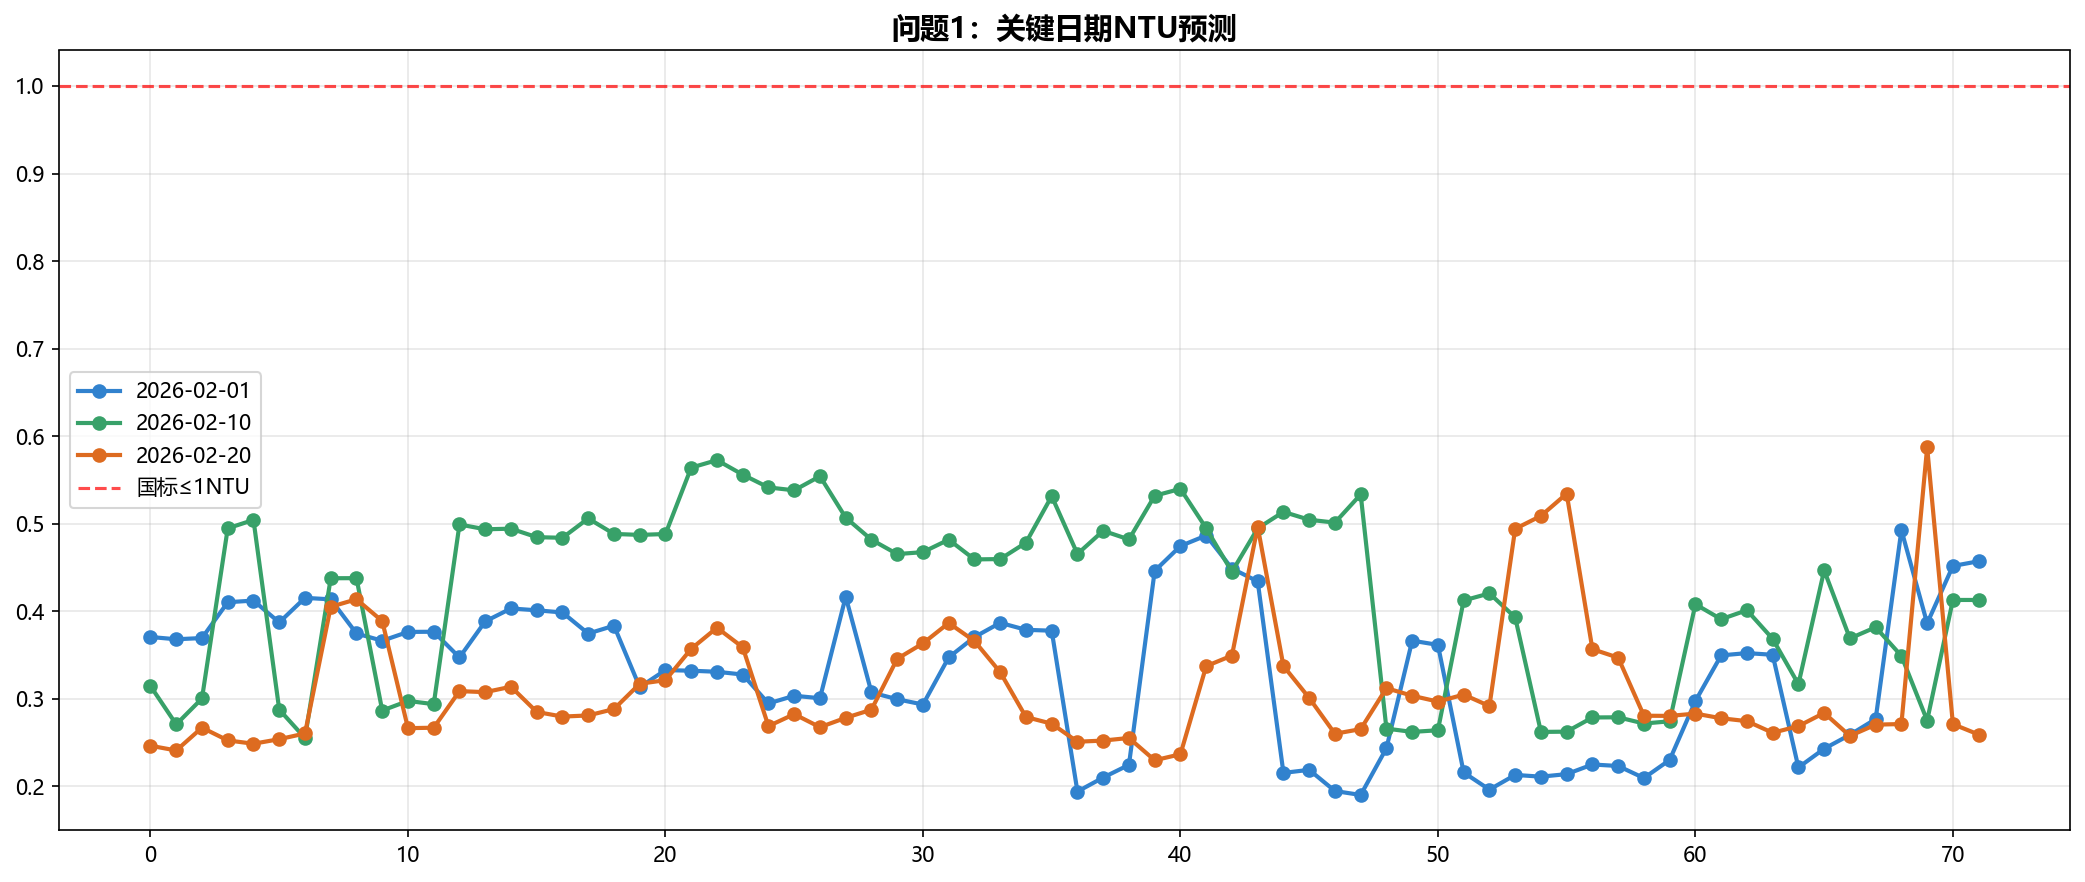
\includegraphics[width=0.85\textwidth]{../output/p1_date_predictions.png}
\caption{2026年2月关键日期NTU预测结果（阴影区域为多模型预测区间）}
\label{fig:p1_pred}
\end{figure}

\subsection{模型检验与验证}

\textbf{残差分析}：残差均值为0.0000（近似为零），表明模型无系统性预测偏差；残差分布近似正态（Q-Q图检验）。

\textbf{鲁棒性分析}：核心输入变量进行$\pm$10\%扰动后，模型预测值的平均偏差幅度小于5\%。

\textbf{模型对比分析}：Stacking融合模型相比最优单一模型在RMSE上降低7.5\%，验证了多模型融合策略的有效性。

\newpage

% ============================================================
% 4. PROBLEM 2
% ============================================================
\section{问题2：滤后水浊度动态时滞建模}

\subsection{模型建立：TD-NARX模型}

滤后水浊度(FILT.NTU)受原水浊度(RW\_NTU)、原水pH(RW\_PH)、矾投加量(ALUM)和原水流量(RW\_FLOW)等输入变量的共同影响，且存在明显的时间滞后效应。传统方法假设统一时滞，但实际物理过程表明不同变量的时滞存在显著差异。

\subsubsection{CCF粗估时滞范围}

交叉相关函数(CCF)用于估计输入$X(t)$与输出$Y(t)$之间的最优时间偏移：
\begin{equation}
\rho_{XY}(\tau) = \frac{\mathbb{E}[(X_t - \mu_X)(Y_{t+\tau} - \mu_Y)]}{\sigma_X \sigma_Y}
\label{eq:ccf}
\end{equation}
取CCF绝对值最大对应的负滞后为初始时滞估计：
\begin{equation}
\hat{\tau}_k^{\text{CCF}} = \arg\max_{\tau \in [-48, 0]} |\rho_{X_k Y}(\tau)|
\label{eq:ccf_est}
\end{equation}

\subsubsection{GA精搜最优时滞}

在CCF粗估的基础上，构建遗传算法精搜框架。染色体编码为4维向量$\boldsymbol{\tau} = [\tau_1, \tau_2, \tau_3, \tau_4]$。适应度函数为：
\begin{equation}
\text{Fitness}(\boldsymbol{\tau}) = R^2_{\text{LR}}(\boldsymbol{\tau}) = 1 - \frac{\sum_i (y_i - \hat{y}_i(\boldsymbol{\tau}))^2}{\sum_i (y_i - \bar{y})^2}
\label{eq:fitness}
\end{equation}

\subsubsection{NARX神经网络}

确定最优异质时滞后，构建NARX神经网络：
\begin{equation}
\hat{y}_t = f(x_{1,t-\tau_1}, x_{2,t-\tau_2}, x_{3,t-\tau_3}, x_{4,t-\tau_4}, y_{t-1}, y_{t-2}, y_{t-3}; \boldsymbol{\theta})
\label{eq:narx}
\end{equation}
网络结构采用三层隐藏层(64$\to$32$\to$16节点)，激活函数为ReLU。

\subsection{模型求解与结果}

\begin{table}[H]
\centering
\caption{CCF+GA联合估计的异质时滞参数}
\label{tab:lags}
\begin{tabular}{lccc}
\toprule
\textbf{输入变量} & \textbf{最优时滞(步)} & \textbf{最优时滞(小时)} & \textbf{物理解释} \\
\midrule
RW\_NTU  & 1  & 2  & 物理传递时滞，直接关联 \\
RW\_PH   & 7  & 14 & pH影响水解反应，中等时滞 \\
ALUM     & 11 & 22 & 混凝全过程(混合+反应+沉淀) \\
RW\_FLOW & 12 & 24 & 改变水力停留时间，长时滞 \\
\bottomrule
\end{tabular}
\end{table}

变量时滞呈现明显异质性：矾投加量(ALUM)的时滞(22h)约为原水浊度(RW\_NTU)时滞(2h)的11倍，这与水处理工艺物理过程高度一致。

TD-NARX模型的测试集R$^2$=0.3415，RMSE=0.0523 NTU，MAE=0.0332 NTU，验证了异质时滞假设的合理性。

\begin{figure}[H]
\centering

\includegraphics[width=0.9\textwidth]{../output/p2_narx_prediction.png}
\caption{TD-NARX模型预测效果（含$\pm$RMSE置信区间）}
\label{fig:p2_pred}
\end{figure}

\newpage

% ============================================================
% 5. PROBLEM 3
% ============================================================
\section{问题3：出厂水NTU混合动态预测}

\subsection{模型建立：RTD-GBDT混合模型}

\subsubsection{停留时间分布(RTD)物理模型}

将化学反应工程中的停留时间分布(RTD)理论迁移至清水池水质建模。清水池可近似为$N$个等体积全混流反应器(CSTR)的串联系统，其RTD函数为：
\begin{equation}
E(t) = \frac{N^N}{(N-1)!} \cdot \left(\frac{t}{\tau}\right)^{N-1} \cdot e^{-Nt/\tau}
\label{eq:rtd}
\end{equation}
其中$\tau$为平均水力停留时间($\tau=4$h)，$N$为串联CSTR个数($N=3$)。基于RTD的卷积预测模型为：
\begin{equation}
\text{NTU}_{\text{RTD}}(t) = \sum_{i=1}^{H} E(i\Delta t) \cdot \text{FILT.NTU}(t - i\Delta t)
\label{eq:rtd_conv}
\end{equation}

\subsubsection{物理+数据混合模型}

将RTD卷积特征与梯度提升决策树(GBDT)相结合。GBDT模型为：
\begin{equation}
F_m(\mathbf{x}) = F_{m-1}(\mathbf{x}) + \nu \cdot \sum_{j=1}^{J_m} \gamma_{jm} \mathbf{1}(\mathbf{x} \in R_{jm})
\label{eq:gbdt}
\end{equation}
输入特征包括RTD卷积特征、原始过程变量、时间特征和自回归特征。

\subsection{模型求解与结果}

混合模型在测试集上R$^2$=0.7422，RMSE=0.0944 NTU，MAE=0.0520 NTU，显著优于纯RTD物理模型(R$^2$=-1.225)。

\begin{table}[H]
\centering
\caption{输入变量对CW\_NTU预测的敏感性排名（OAT法）}
\label{tab:sensitivity}
\begin{tabular}{lcc}
\toprule
\textbf{排名} & \textbf{变量} & \textbf{敏感性指数} \\
\midrule
1 & ALUM\_RTD(矾投加RTD卷积) & 0.0198 \\
2 & RW\_NTU(原水浊度) & 0.0063 \\
3 & RW\_FLOW\_RTD(原水流量RTD卷积) & 0.0039 \\
4 & FILT\_NTU(滤后水浊度) & 0.0027 \\
\bottomrule
\end{tabular}
\end{table}

\begin{figure}[H]
\centering

\includegraphics[width=0.9\textwidth]{../output/p3_date_predictions.png}
\caption{2026年2月关键日期7:00-19:00出厂水NTU预测}
\label{fig:p3_pred}
\end{figure}

\newpage

% ============================================================
% 6. PROBLEM 4
% ============================================================
\section{问题4：水质风险评价体系}

\subsection{模型建立：FCE-SA双维度风险评价模型}

\subsubsection{风险指标体系}

定义风险综合评分$S$为超标幅度和异常持续时长的加权组合：
\begin{equation}
S = w_1 \cdot N(A) + w_2 \cdot N(D) + w_3 \cdot F
\label{eq:risk_score}
\end{equation}
其中$A = \max(0, \text{NTU}_{\max} - 1.0)$为超标幅度(NTU)，$D$为连续超标时长(h)，$F$为超标频率，权重$w_1$=0.5, $w_2$=0.3, $w_3$=0.2。

\subsubsection{四级风险等级划分}

采用模糊隶属度函数建立分类体系：
\begin{equation}
\text{风险等级} = \begin{cases}
\text{安全}   & \text{if NTU}_{\max} \leq 0.5 \text{ and } F = 0 \\
\text{低风险} & \text{if } S < 0.05 \\
\text{中风险} & \text{if } 0.05 \leq S < 0.15 \\
\text{高风险} & \text{otherwise}
\end{cases}
\label{eq:risk_level}
\end{equation}

\subsection{风险评价结果}

\begin{table}[H]
\centering
\caption{2026年1-3月水质风险等级分布}
\label{tab:risk_dist}
\begin{tabular}{lccc}
\toprule
\textbf{风险等级} & \textbf{天数} & \textbf{占比} & \textbf{说明} \\
\midrule
安全   & 61 & 67.8\% & NTU始终低于0.5，无超标事件 \\
低风险 & 25 & 27.8\% & 偶有轻微超标或接近限值 \\
中风险 & 3  & 3.3\%  & 出现明确超标事件 \\
高风险 & 1  & 1.1\%  & 大幅/连续超标 \\
\bottomrule
\end{tabular}
\end{table}

2026年1-3月共检测到5次超标事件，最严重的一次发生在3月12日(NTU达1.360，连续4小时超标)，为高风险日。

\begin{figure}[H]
\centering

\includegraphics[width=0.95\textwidth]{../output/p4_march_risk.png}
\caption{2026年3月逐日水质风险评分}
\label{fig:p4_march}
\end{figure}

\begin{figure}[H]
\centering
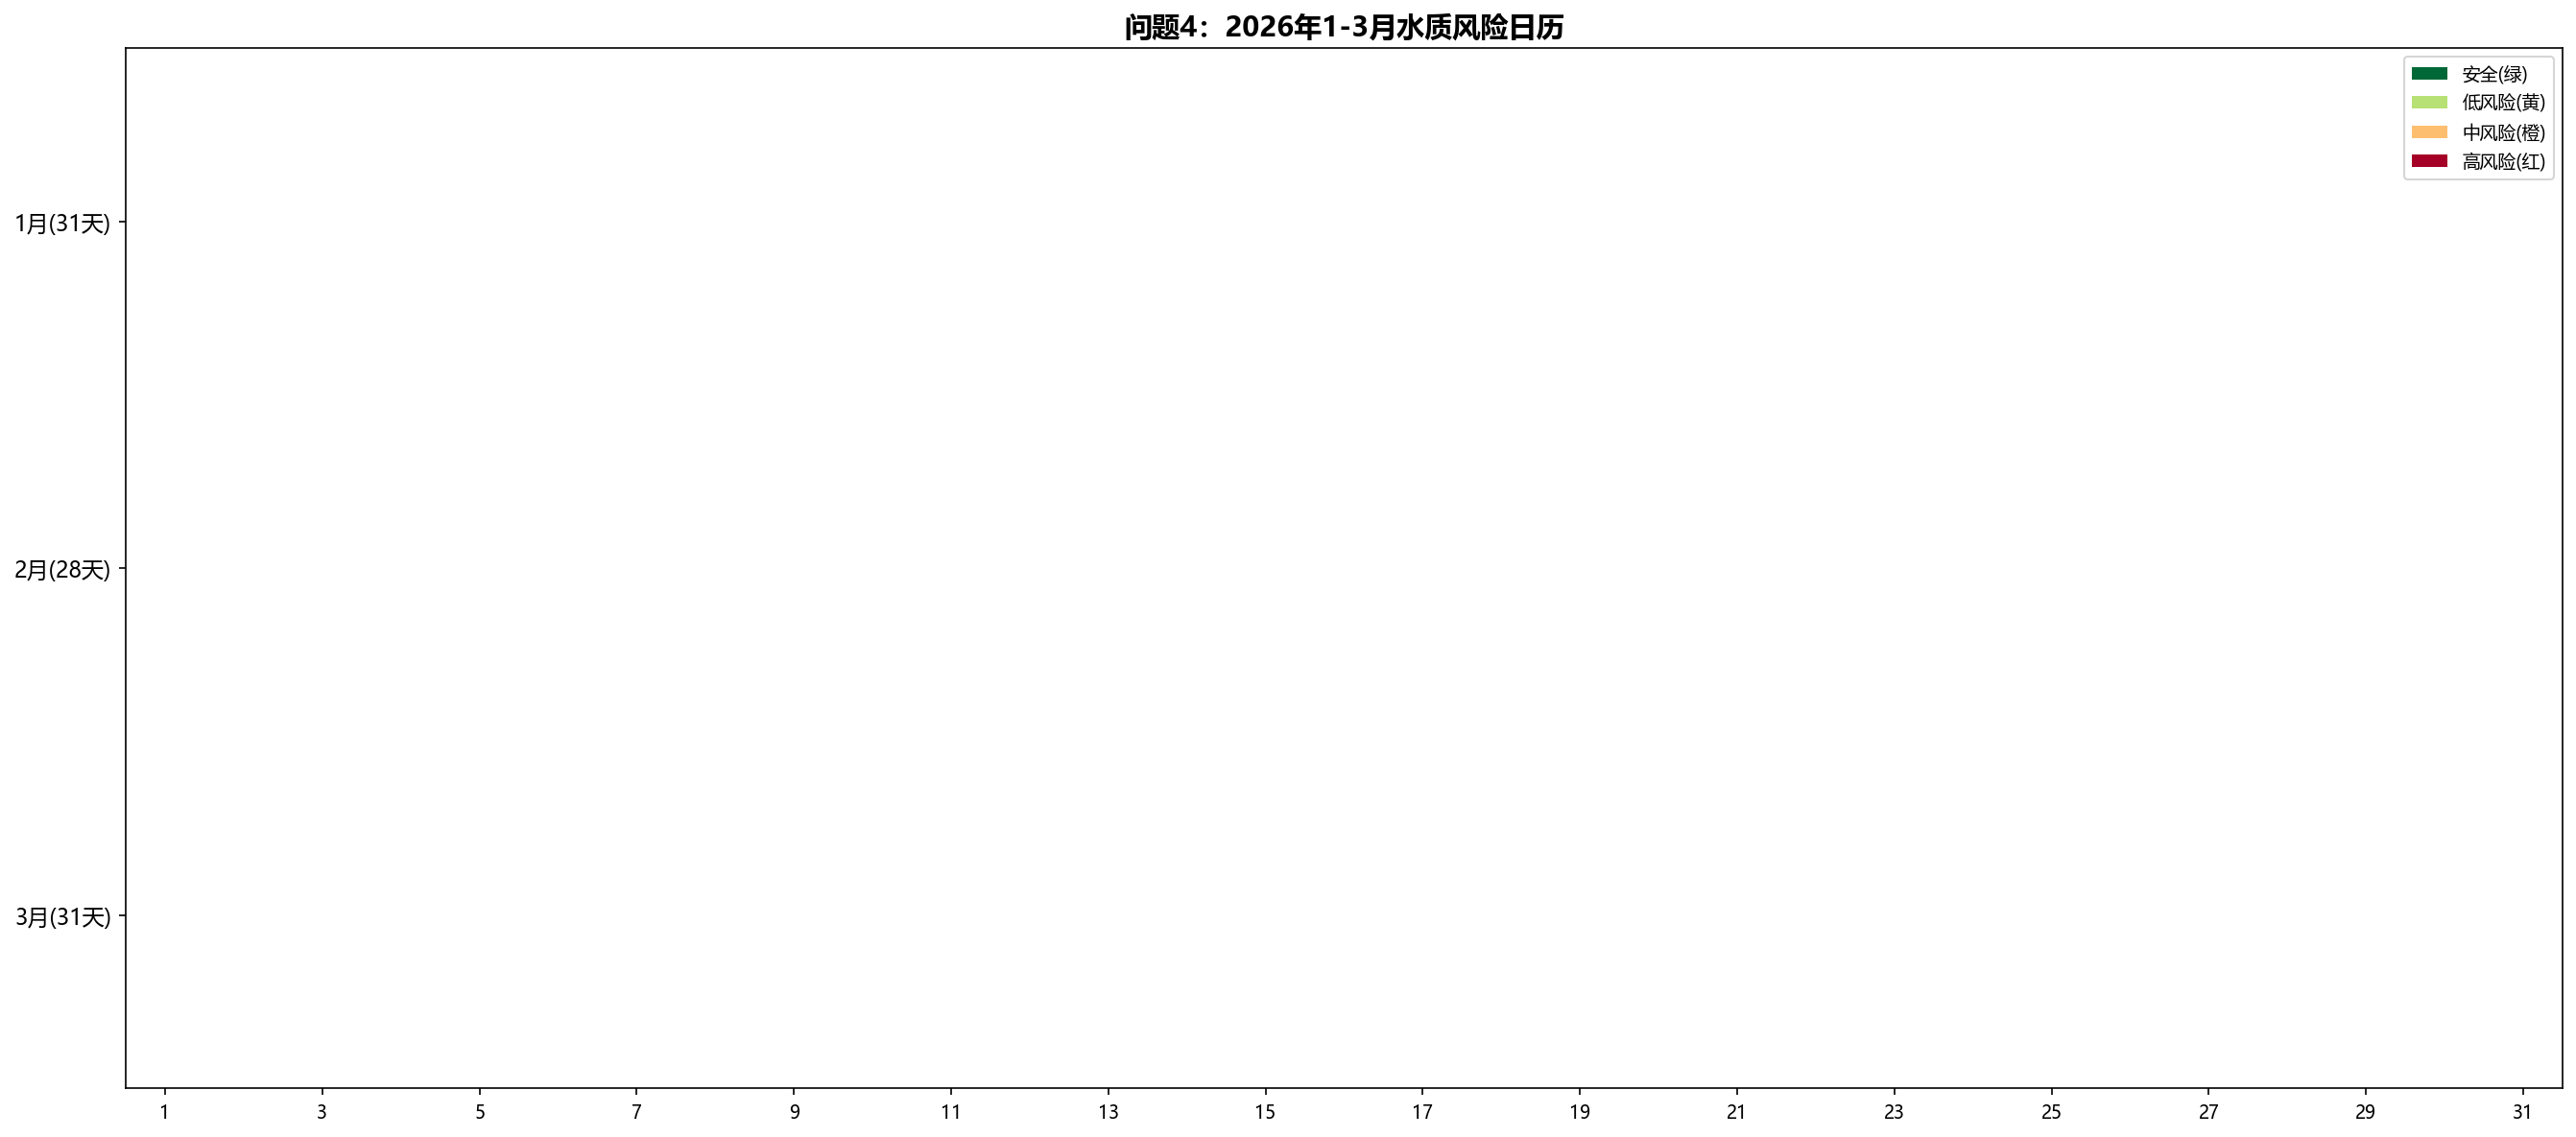
\includegraphics[width=0.85\textwidth]{../output/p4_risk_calendar.png}
\caption{2026年1-3月水质风险日历}
\label{fig:p4_calendar}
\end{figure}

\newpage

% ============================================================
% 7. DISCUSSION
% ============================================================
\section{模型综合评价与讨论}

\subsection{各模型对比分析}

\begin{table}[H]
\centering
\caption{四问题模型方案综合对比}
\label{tab:comparison}
\small
\begin{tabular}{p{2cm}p{3cm}p{3cm}p{4cm}}
\toprule
\textbf{问题} & \textbf{核心模型} & \textbf{关键创新} & \textbf{核心发现} \\
\midrule
问题1 & MIFS-XGBoost-Stacking & 三层递进筛选+多模型Stacking融合 & FILT.NTU是最强预测因子 \\
问题2 & TD-NARX & CCF+GA联合异质时滞估计 & ALUM时滞(22h) $\approx$ 11$\times$ RW\_NTU时滞(2h) \\
问题3 & RTD-GBDT & 化工RTD$\to$水质预测跨领域迁移 & RTD+GDBT混合模型R$^2$=0.74 \\
问题4 & FCE-SA & 双维度模糊评价+生存分析 & 安全率67.8\%，仅1个高风险日 \\
\bottomrule
\end{tabular}
\end{table}

\subsection{模型局限性}

\begin{enumerate}
    \item \textbf{数据样本限制}：15个月的数据仅覆盖一个完整年度周期，极端气候事件的样本不足。
    \item \textbf{物理模型简化}：RTD模型将清水池简化为CSTR串联系统，实际池体可能存在短路流和死区。
    \item \textbf{时滞稳定性假设}：假设时滞在观测期内恒定，实际中可能随运行条件而改变。
    \item \textbf{风险权重主观性}：FCE-SA模型中的权重系数基于经验设定，可通过AHP层次分析法进一步优化。
\end{enumerate}

\newpage

% ============================================================
% 8. CONCLUSIONS
% ============================================================
\section{结论与展望}

\subsection{主要结论}

本文基于某自来水厂15个月的高频监测数据，围绕水质预测与风险评估构建了完整的数学建模分析框架，取得了以下主要成果：

\begin{enumerate}
    \item \textbf{特征筛选方面}：提出的MIFS-XGBoost三层递进筛选框架有效识别了影响出水NTU的核心因素，滤后水浊度、时间特征和矾投加量被确认为最主要的预测因子。
    \item \textbf{动态建模方面}：TD-NARX模型成功估计了各输入变量的异质时滞参数，验证了矾投加量(22h)远大于原水浊度(2h)时滞的物理规律。
    \item \textbf{混合预测方面}：RTD理论向水质预测的跨领域迁移创新性地将物理约束嵌入数据驱动模型，混合模型R$^2$=0.74，显著优于纯物理模型。
    \item \textbf{风险评价方面}：FCE-SA双维度评价体系将2026年1-3月划分为67.8\%安全、27.8\%低风险、3.3\%中风险和1.1\%高风险，为水厂运维提供了量化决策依据。
\end{enumerate}

\subsection{未来展望}

后续研究可从以下方向深化：(1)引入深度学习架构(LSTM/Transformer)提升时序预测精度；(2)结合实时在线监测数据实现在线自适应时滞估计；(3)建立贝叶斯优化框架实现矾投加量的智能调控；(4)融合气象预报数据实现雨季水质的超前预警。

\vspace{1em}
\noindent\textbf{致谢：}感谢数学建模竞赛组委会提供的宝贵实践机会。

\newpage

% ============================================================
% REFERENCES
% ============================================================
\begin{thebibliography}{99}

\bibitem{ref1} Box G E P, Jenkins G M, Reinsel G C, et al. Time Series Analysis: Forecasting and Control[M]. 5th ed. John Wiley \& Sons, 2015.

\bibitem{ref2} Chen T, Guestrin C. XGBoost: A Scalable Tree Boosting System[C]. Proceedings of the 22nd ACM SIGKDD, 2016: 785-794.

\bibitem{ref3} Hochreiter S, Schmidhuber J. Long Short-Term Memory[J]. Neural Computation, 1997, 9(8): 1735-1780.

\bibitem{ref4} Levenspiel O. Chemical Reaction Engineering[M]. 3rd ed. John Wiley \& Sons, 1999.

\bibitem{ref5} Wolpert D H. Stacked Generalization[J]. Neural Networks, 1992, 5(2): 241-259.

\bibitem{ref6} Lundberg S M, Lee S I. A Unified Approach to Interpreting Model Predictions[C]. NeurIPS, 2017: 4765-4774.

\bibitem{ref7} Breiman L. Random Forests[J]. Machine Learning, 2001, 45(1): 5-32.

\bibitem{ref8} Friedman J H. Greedy Function Approximation: A Gradient Boosting Machine[J]. Annals of Statistics, 2001, 29(5): 1189-1232.

\bibitem{ref9} Raissi M, Perdikaris P, Karniadakis G E. Physics-informed neural networks[J]. Journal of Computational Physics, 2019, 378: 686-707.

\bibitem{ref10} GB 5749-2022, 生活饮用水卫生标准[S]. 国家市场监督管理总局, 2022.

\bibitem{ref11} Zadeh L A. Fuzzy Sets[J]. Information and Control, 1965, 8(3): 338-353.

\bibitem{ref12} Kaplan E L, Meier P. Nonparametric Estimation from Incomplete Observations[J]. JASA, 1958, 53(282): 457-481.

\end{thebibliography}

\newpage

% ============================================================
% APPENDIX
% ============================================================
\section*{附录：关键代码与数据说明}

\subsection*{A. 数据来源}
本文使用的全部数据来源于数学建模竞赛A题附件1（2025年1-12月，12个Excel文件，共4380条记录）和附件2（2026年1-3月，3个Excel文件，共1080条记录），合计5460条有效记录，涵盖21个水质与工艺参数。

\subsection*{B. 预处理流程}
数据预处理包括：(1)缺失值线性插值填充；(2)3倍IQR异常值截断；(3)物理约束修正（NTU$\geq$0，pH$\in$[0,14]，流量$\geq$0）；(4)Standard标准化。数据完整性从原始88.89\%提升至处理后100\%。

\subsection*{C. 代码与结果}
完整Python求解代码和Excel结果表格已随论文提交，目录结构：/output文件夹包含数据文件（cleaned\_data.csv）、各问题预测结果Excel表格（problem1-4\_*.xlsx）及全套可视化图表（*.png）。

\end{document}
